\documentclass[a4paper]{article}

\usepackage{inputenc}
\usepackage[british,UKenglish]{babel}
\usepackage{amsmath}
%\usepackage{titlesec}
\usepackage{color}
\usepackage{graphicx}
\usepackage{fancyref}
\usepackage{hyperref}
\usepackage{float}
\usepackage{scrextend}
\usepackage{setspace}
\usepackage{xargs}
\usepackage{multicol}
\usepackage{nameref}

\usepackage{sectsty}
\usepackage{multicol}
\usepackage{multirow}
\usepackage[procnames]{listings}
\usepackage{appendix}

\newcommand\tab[1][1cm]{\hspace*{#1}}
\hypersetup{colorlinks=true, linkcolor=black}
\interfootnotelinepenalty=10000

\newcommand{\cleancode}[1]{\begin{addmargin}[3em]{3em}\texttt{\textcolor{cleanOrange}{#1}}\end{addmargin}}
\newcommand{\cleanstyle}[1]{\text{\textcolor{cleanOrange}{\texttt{#1}}}}


\usepackage[colorinlistoftodos,prependcaption,textsize=footnotesize]{todonotes}
\newcommandx{\commred}[2][1=]{\textcolor{Red}
{\todo[linecolor=red,backgroundcolor=red!25,bordercolor=red,#1]{#2}}}
\newcommandx{\commblue}[2][1=]{\textcolor{Blue}
{\todo[linecolor=blue,backgroundcolor=blue!25,bordercolor=blue,#1]{#2}}}
\newcommandx{\commgreen}[2][1=]{\textcolor{OliveGreen}{\todo[linecolor=OliveGreen,backgroundcolor=OliveGreen!25,bordercolor=OliveGreen,#1]{#2}}}
\newcommandx{\commpurp}[2][1=]{\textcolor{Plum}{\todo[linecolor=Plum,backgroundcolor=Plum!25,bordercolor=Plum,#1]{#2}}}

\def\code#1{{\tt #1}}

\def\note#1{\noindent{\bf [Note: #1]}}

\makeatletter
%% The "\@seccntformat" command is an auxiliary command
%% (see pp. 26f. of 'The LaTeX Companion,' 2nd. ed.)
\def\@seccntformat#1{\@ifundefined{#1@cntformat}%
   {\csname the#1\endcsname\quad}  % default
   {\csname #1@cntformat\endcsname}% enable individual control
}
\let\oldappendix\appendix %% save current definition of \appendix
\renewcommand\appendix{%
    \oldappendix
    \newcommand{\section@cntformat}{\appendixname~\thesection\quad}
}
\makeatother


% "define" Scala
\usepackage[T1]{fontenc}  
\usepackage[scaled=0.82]{beramono}  
\usepackage{microtype} 

\sbox0{\small\ttfamily A}
\edef\mybasewidth{\the\wd0 }

\lstdefinelanguage{scala}{
  morekeywords={abstract,case,catch,class,def,%
    do,else,extends,false,final,finally,%
    for,if,implicit,import,match,mixin,%
    new,null,object,override,package,%
    private,protected,requires,return,sealed,%
    super,this,throw,trait,true,try,%
    type,val,var,while,with,yield},
  sensitive=true,
  morecomment=[l]{//},
  morecomment=[n]{/*}{*/},
  morestring=[b]",
  morestring=[b]',
  morestring=[b]"""
}

\usepackage{color}
\definecolor{dkgreen}{rgb}{0,0.6,0}
\definecolor{gray}{rgb}{0.5,0.5,0.5}
\definecolor{mauve}{rgb}{0.58,0,0.82}

% Default settings for code listings
\lstset{frame=tb,
  language=scala,
  aboveskip=3mm,
  belowskip=3mm,
  showstringspaces=false,
  columns=fixed, % basewidth=\mybasewidth,
  basicstyle={\small\ttfamily},
  numbers=none,
  numberstyle=\footnotesize\color{gray},
  % identifierstyle=\color{red},
  keywordstyle=\color{blue},
  commentstyle=\color{dkgreen},
  stringstyle=\color{mauve},
  frame=single,
  breaklines=true,
  breakatwhitespace=true,
  procnamekeys={def, val, var, class, trait, object, extends},
  procnamestyle=\ttfamily\color{red},
  tabsize=2
}

\lstnewenvironment{scala}[1][]
{\lstset{language=scala,#1}}
{}
\lstnewenvironment{cpp}[1][]
{\lstset{language=C++,#1}}
{}
\lstnewenvironment{bash}[1][]
{\lstset{language=bash,#1}}
{}
\lstnewenvironment{verilog}[1][]
{\lstset{language=verilog,#1}}
{}



\lstset{frame=,basicstyle={\footnotesize\ttfamily}}

\graphicspath{ {images/} }
\usepackage{ctex}
\usepackage{verbatim}
\usepackage{enumerate}
\usepackage{geometry}
\usepackage{amssymb}
\usepackage{amsmath}
%\usepackage{slashbox}
\usepackage{diagbox}
\usepackage{pifont}%\ding{192} \ding{172}
\usepackage{tikz}
\usepackage{booktabs}
\usepackage{float}
\usepackage{bm}
%\geometry{a4paper, scale=0.72}
\geometry{a4paper,left=2.5cm,right=2.5cm,top=2.5cm,bottom=2.5cm}
%%%%%%%%%%%%%%%%%%%%%%%%%%%%%%%%%%%%%%%% BEGIN DOC %%%%%%%%%%%%%%%%%%%%%%%%%%%%%%%%%%%%%%%%

\begin{document}
\setlength{\abovecaptionskip}{0pt}
\setlength{\belowcaptionskip}{0pt}
\renewcommand{\contentsname}{目\ 录}
\renewcommand{\appendixname}{附录}
\renewcommand{\appendixpagename}{附录}
\renewcommand{\refname}{参考文献} 
\renewcommand{\figurename}{图}
\renewcommand{\tablename}{表}
\renewcommand{\today}{\number\year 年 \number\month 月 \number\day 日}
\renewcommand{\comma}{$\mkern -8.5mu\raise -.2ex\hbox{\rotatebox[]{180}{\`}}\ $}

\newcommand*{\circled}[1]{\lower.7ex\hbox{\tikz\draw (0pt, 0pt)%
    circle (.5em) node {\makebox[1em][c]{\small #1}};}}
\title{{\Huge 近代物理实验报告{\large\linebreak\\}}{\Large 实验2-4:\ 康普顿散射\linebreak\linebreak}}
%please write your name, Student #, and Class # in Authors, student ID, and class # respectively
\author{\\姓\ 名:付\ 大\ 为\\
学\ 号: 1800011105\\
邮\ 箱: \url{fudw@pku.edu.cn}\\
%班\ 号: xxxxx\\\\
近代物理实验 (I)\\
(2021,秋季学期)\\\\
北京大学\\
物理学院\\
2018级1班}
\date{\today}
\maketitle
\newpage

%%%%%%%%%%%%%%%%%%%%%%%%%%%%%%%%%%%%%%%% ABSTRACT %%%%%%%%%%%%%%%%%%%%%%%%%%%%%%%%%%%%%%%%
\begin{center}
{\Large\bf{摘\ 要\\}}
\end{center}

康普顿效应源于电子对高能光子的非弹性散射。光的经典波动理论难以解释这一
现象,它强烈地依赖于波粒二象性。本实验以$\mathrm \sideset{^{137}}{}Cs$为放射源,测定了$\rm 662keV\ \gamma$ 射线被铝棒散射后的能量及相对微分散射截面,考察了其关于散射角的分布。实验结果表明,散射光子能量及相对微分散射截面均随散射角增大而递减,其规律与理论分析基本一致,从而验证了康普顿效应,进而证实了光的波粒二象性。\\\\
{\bf{关键词}:}康普顿散射, 能谱, 散射截面
\newpage

%%%%%%%%%%%%%%%%%%%%%%%%%%%%%%%%%%%%%%%% CONTENT %%%%%%%%%%%%%%%%%%%%%%%%%%%%%%%%%%%%%%%%
\begin{center}
\tableofcontents\label{c}
\end{center}
\newpage

%%%%%%%%%%%%%%%%%%%%%%%%%%%%%%%%%%%%%%%% Introduction %%%%%%%%%%%%%%%%%%%%%%%%%%%%%%%%%%%%%%%%
\section{引言} \label{overview}%------------------------------
20 世纪早期,诸多实验迹象表明,被物质散射后的 X 射线能量减小1;而经典电动力学的预测表明,散射波的能量应当与入射波一致。

1923 年,康普顿(A. H. Compton)采用光量子假定,结合狭义相对论的动力学,成功地解释了散射能量的变化。据此理论可知,光子的能量损失源于与电子的非弹性散射;其有效性在吴有训等人的一系列后续实验被进一步加以证实。

康普顿散射进一步确认了光子正是传递电磁场相互作用的粒子(force carrier)。1928 年,Oskar Klein 和 Yoshita Nishina 根据狄拉克(Paul Dirac)的量子电动力学(QED)推导出了散射的微分截面。Klein–Nishina 公式是 QED 的最早成果之一,其在低能极限下表征经典的弹性散射(汤姆逊散射),而在高能情形下对应康普顿散射。

如今,康普顿散射仍作为研究基本粒子结构的一个重要方法。本实验意在复现康普顿效应的验证过程,通过测定$\gamma$射线的能谱,分析能量及相对微分散射截面随散射角$\theta$的变化,以验证上述理论结果。这也是对吴先生的工作的一次重现。

%%%%%%%%%%%%%%%%%%%%%%%%%%%%%%%%%%%%%%%% Theory %%%%%%%%%%%%%%%%%%%%%%%%%%%%%%%%%%%%%%%%
\newpage
\section{理论} \label{theory}%------------------------------
考虑高能极限,即光子能量远大于电子束缚能,此时电子近似是自由的;由相对论性能动量守恒,光子能量$e = h\nu$, 可得:
\begin{equation}
	h\nu' = \frac{h\nu}{1 + \frac{h\nu}{mc^2}\pqty{1 - \cos\theta}}
\end{equation}

这里,$m \sim \SI{.511}{\MeV/c^2}$是电子的静质量,$\nu,\nu'$是散射前后光子的频率变化,$h$为普朗克常数,$c$为光速。

Klein--Nishina公式给出关于立体角元$\Omega$的微分散射截面:
\begin{equation}
\begin{aligned}
	\frac{d\sigma}{d\Omega}= r_0^2&\left[\frac{1}{1+\alpha\,(1-\cos \theta )}\right]^2\left(\frac{1+\cos ^2\theta}{2}\right)\left[1+\frac{\alpha ^2 (1-\cos\theta)^2}{\pqty\big{(1+\cos^2\theta)}[\pqty\big{1+\alpha\,(1-\cos \theta)]}}\right]
\end{aligned}
\end{equation}

这里采用了给出的形式,其中$r_0 \sim\SI{2.818}{fm}$为电子的经典半径,$\alpha = \frac{h\nu}{mc^2}$. 
	
考虑实测过程,微分散射截面可表示为:
\begin{equation}
	\frac{d\sigma}{d\Omega}\propto \frac{N(\theta)}{R(E)\,\eta(E)},\quad E = E(\theta)
\end{equation}

$N(\theta)$为实测光电峰值计数;由于存在显著的本底,这里\cjkdot{约定}峰的区间为峰值附近、计数$>\frac{1}{3}$峰值的区域.

此外,峰总比$R(e)$及探测效率$\eta(e)$是探测器的属性,它们是能量$E$的函数,从而间接依赖于$\theta$,比例系数不依赖于散射角$\theta$;

这里我们关注微分散射截面随$\theta$的变化规律,则关注相对微分散射截面即可:
\begin{equation}
    \frac{d\sigma(\theta)}{d\Omega}\bigg/\frac{d\sigma(\theta_0)}{d\Omega}=\frac{N_p(\theta)}{R(\theta)\eta(\theta)}\bigg/\frac{N_p(\theta_0)}{R(\theta_0)\eta(\theta_0)}
\end{equation}
	

%%%%%%%%%%%%%%%%%%%%%%%%%%%%%%%%%%%%%%%% Experiment %%%%%%%%%%%%%%%%%%%%%%%%%%%%%%%%%%%%%%%%
\newpage
\section{实验} \label{experiment}%------------------------------

\subsection{实验仪器}
\begin{enumerate}[(1)]
    \item 康普顿散射实验台一套:含台面主架、导轨、铅屏蔽块及散射用铝棒$(\phi=20mm)$.
    \item 放射源:一个约10mCi的$\mathrm{\sideset{^{137}}{}Cs}$放射源,密封安装在铅室屏蔽体内;作刻度用的$\mathrm{\sideset{^{60}}{}Co}$放射源一个及小铅盒.
    \item 闪烁探测器:NaI晶体为$\phi 40 \times40mm$;光电倍增管型号为CRI05.
    \item 多道一体机一台:含高、低压电源,主放大器,ADC.
    \item 电脑一台:含UMS或PHA仿真软件
\end{enumerate}

\begin{comment}
\subsection{简要实验步骤}\label{sub:ExperimentalSteps}
\begin{enumerate}[1.]
    \item 连接实验装置.先用脉冲发生器作输入信号源,用示波器观察各级输出,调节放大倍数,使得线性放大器输出的脉冲幅度为5~6V.
    \item 用示波器观察
    \item
    \item
\end{enumerate}

\circled{1}抽真空(按橘色按钮),约2分钟,机械泵声音平稳即可\\\\
\end{comment}
%%%%%%%%%%%%%%%%%%%%%%%%%%%%%%%%%%%%%%%% Results & Discussions %%%%%%%%%%%%%%%%%%%%%%%%%%%%%%%%%%%%%%%%
\newpage
\section{结果及分析}

%------------------------------------------------------------
\subsection{做能量刻度(取下散射棒,在$\theta=0^{\circ}$时测量)}\label{sub1}
\begin{enumerate}[1)]
\item 打开$\mathrm \sideset{^{137}}{}Cs$源,调节探头高压$\rm HV=520V$,预热10分钟,调节放大GAIN ADJ约为3.3左右,测量时间设置为600s(后面的策略时间均为600s不变),使 0.662MeV光电峰落在480道左右,测量其全谱,通过寻峰定出全能峰(0.662MeV)对应的准确道数.
\item 关闭$\mathrm \sideset{^{137}}{}Cs$源,放上$\mathrm \sideset{^{60}}{}Co$源(尽量靠近NaI探头),测量其全能谱,定出1.17MeV和1.33MeV两峰对应的准确道数.
\item 根据测得的三个峰,做能量刻度(用最小直线二乘法),刻度如下\textbf{图\ref{fig:fig1}}.
\begin{figure}[H]
 \centering
 \caption{$\theta=0^{\circ}$的能量刻度}
 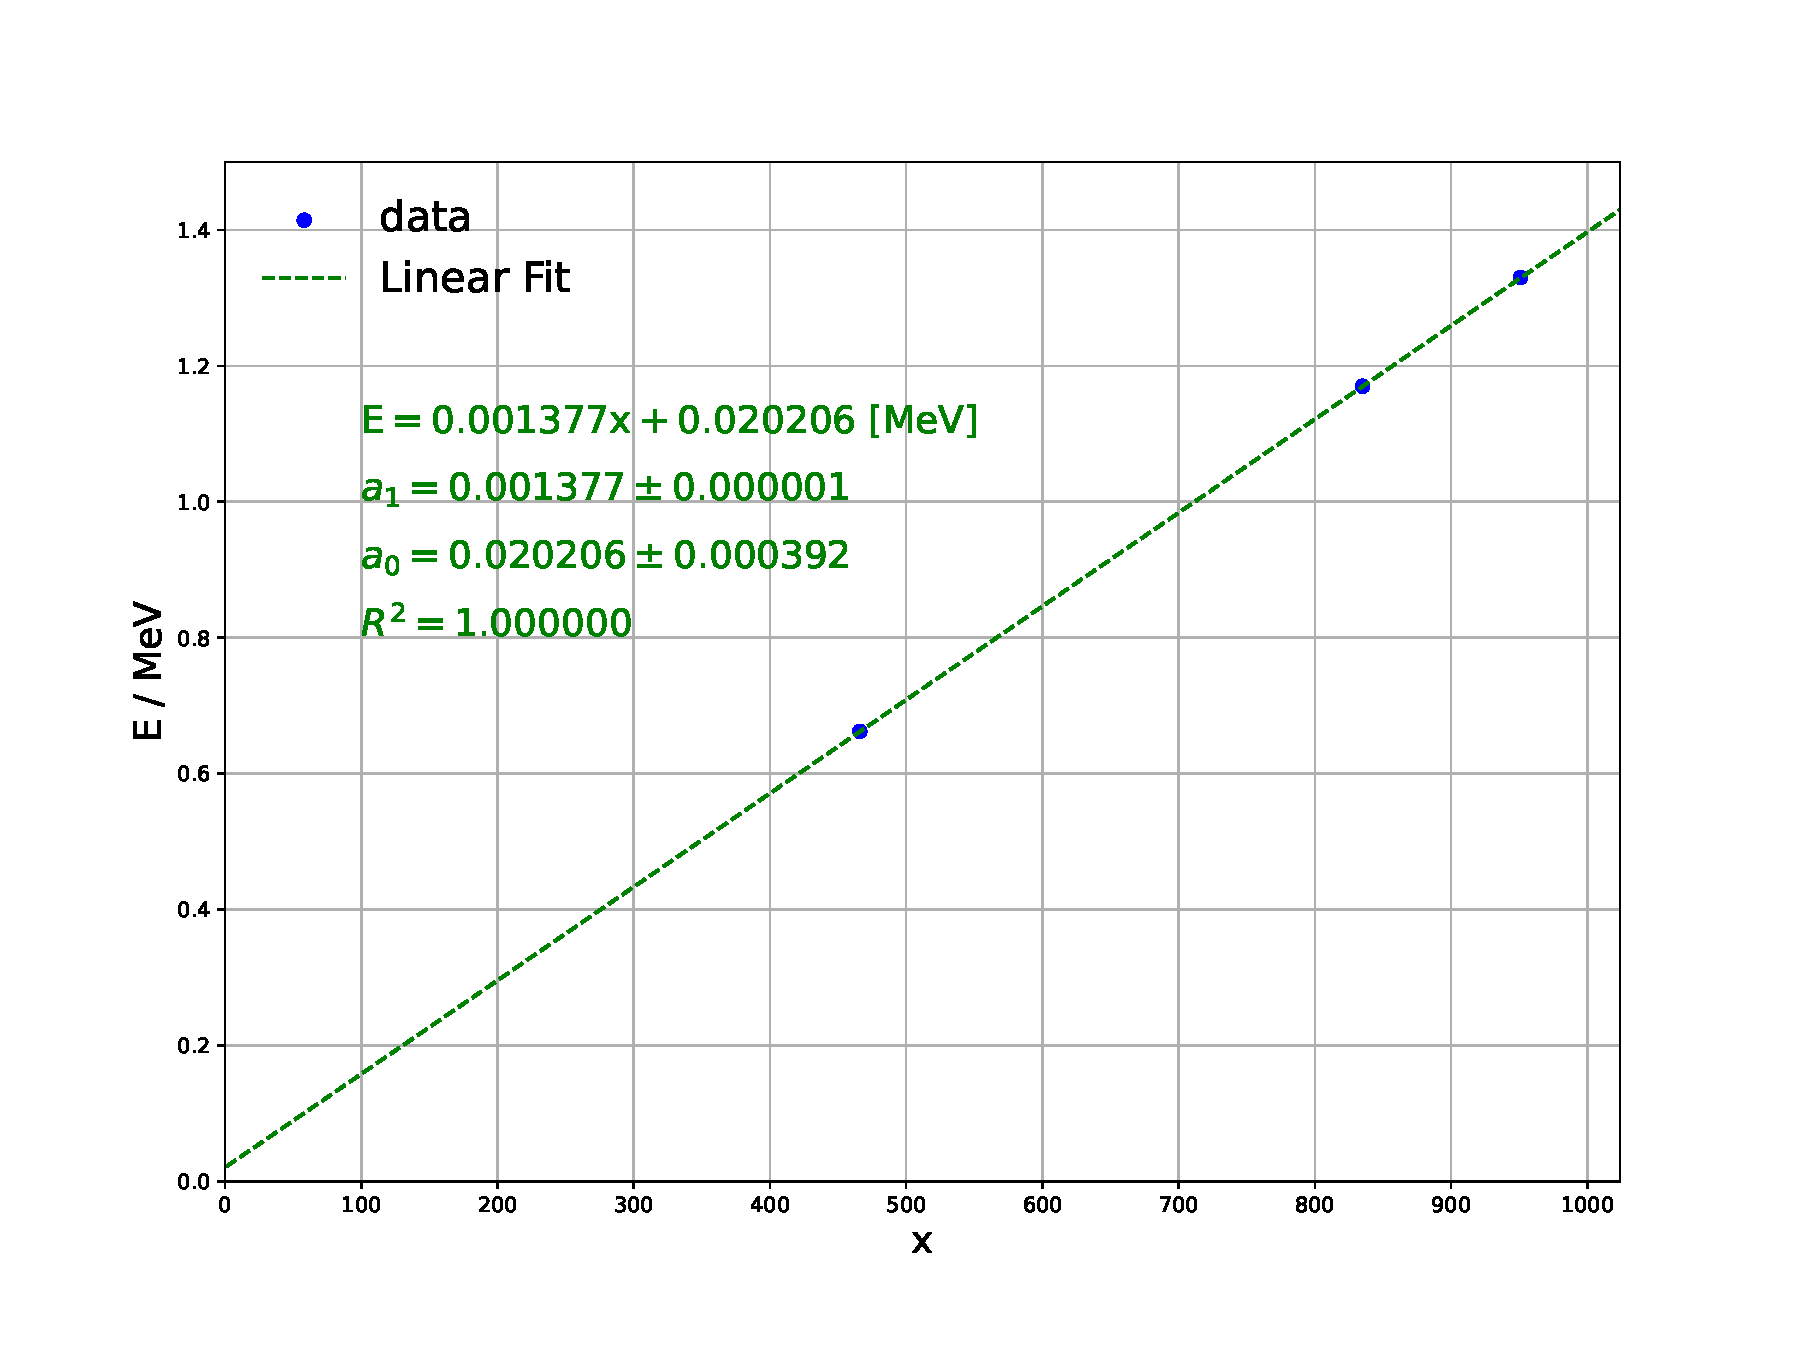
\includegraphics[height=12cm, width=16cm]{images/phyex1_fig.pdf}
 \label{fig:fig1}
\end{figure}\\\\
\end{enumerate}

%------------------------------------------------------------
\subsection{安装散射棒,打开$\mathrm \sideset{^{137}}{}Cs$源(注意: 放射源全部打开)}\label{sub2}
测量微分散射截面和散射峰随散射角的变化.散射角分别取: $\theta=20^{\circ},40^{\circ},60^{\circ},80^{\circ},100^{\circ},120^{\circ}$通过操作“寻峰”和“重点区计算”键,找出并记录下光电峰的峰位、左右光标道址(峰值的三分之一处),重点区面积,测量能谱如下\textbf{图\ref{fig:fig6}}.
\begin{figure}[H]
 \centering
 \caption{$\mathrm \sideset{^{137}}{}Cs$源光子被铝棒散射后的能谱}
 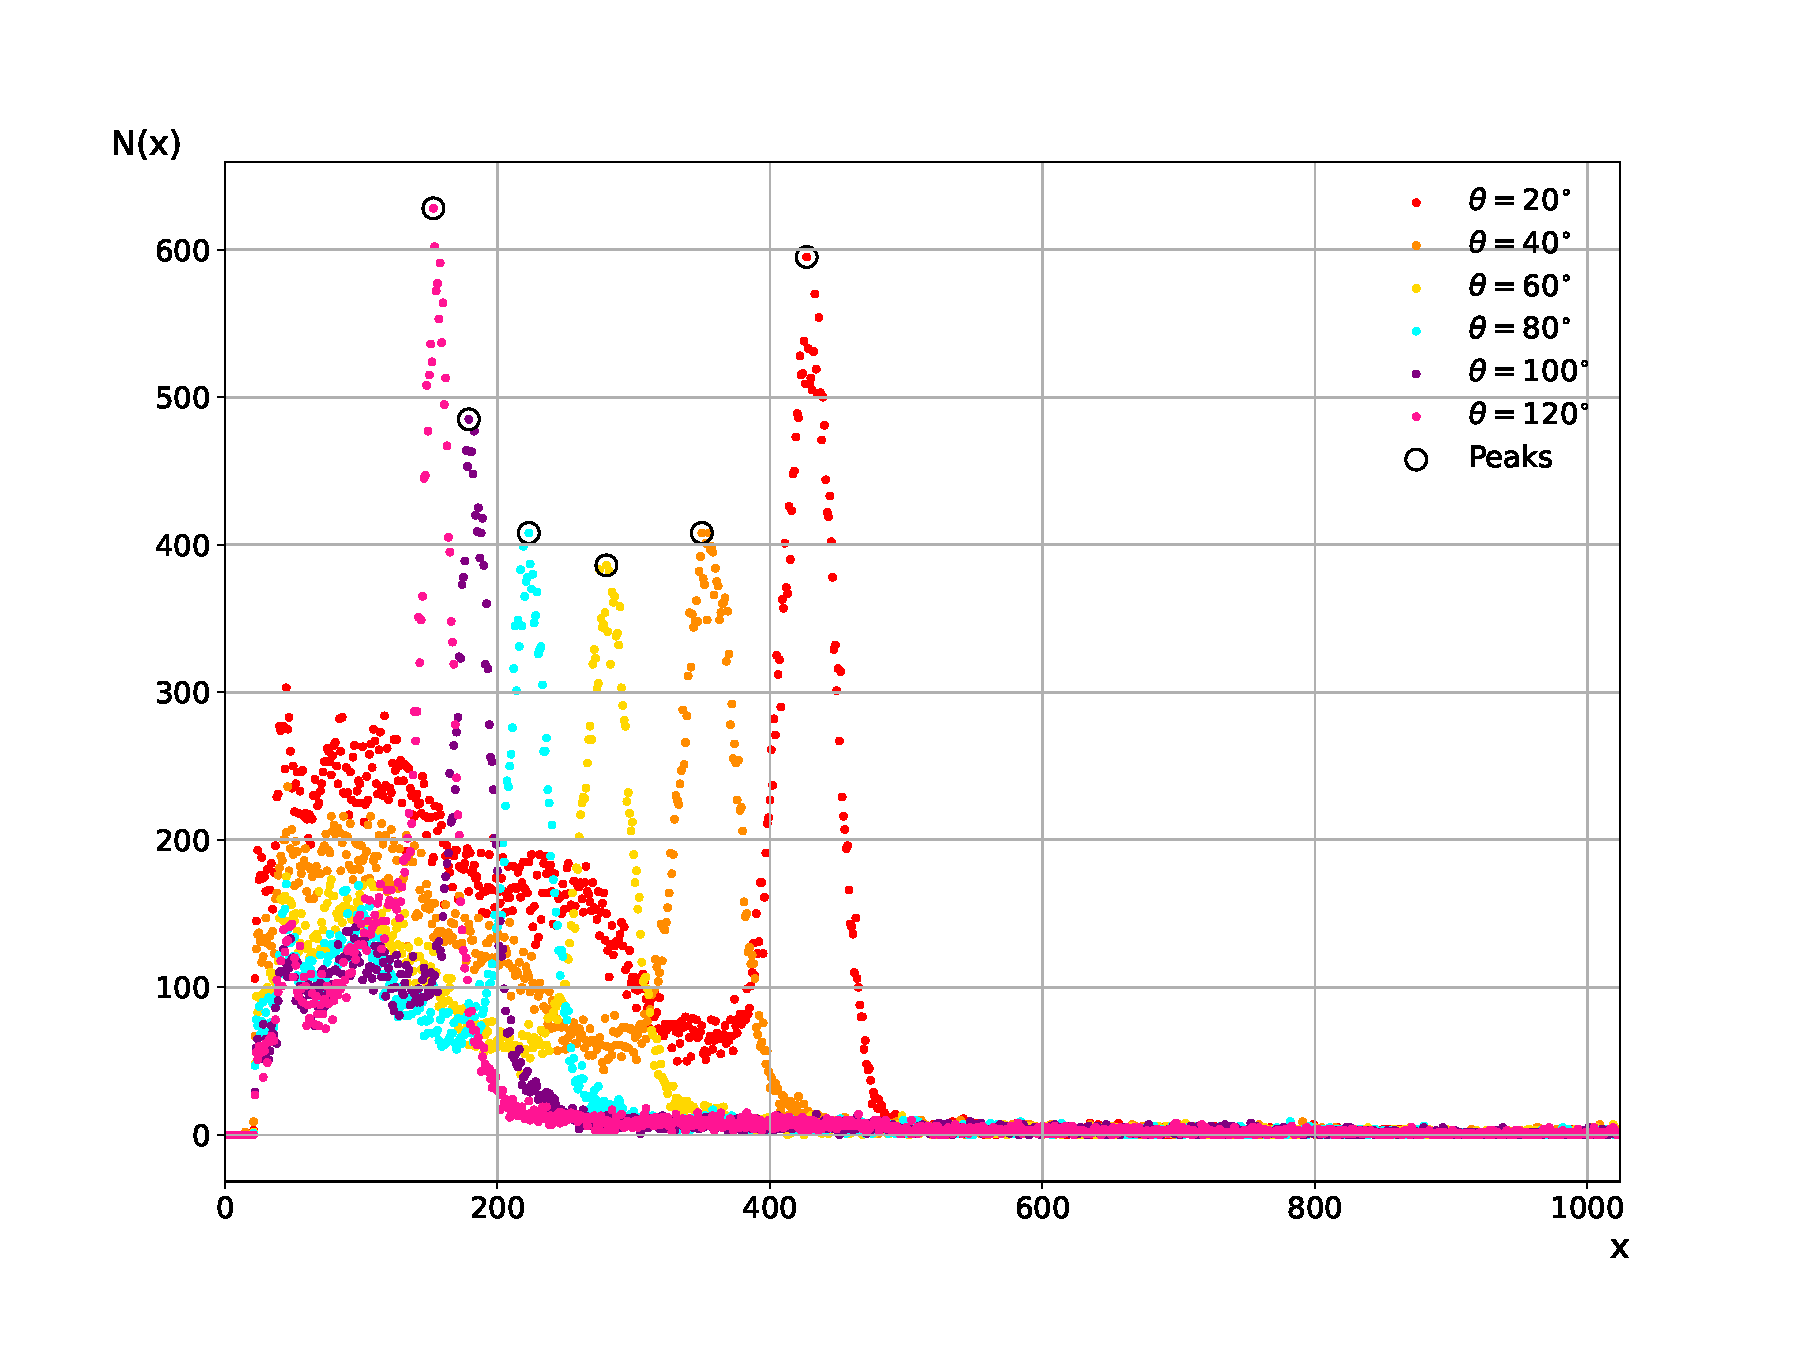
\includegraphics[height=12cm, width=16cm]{images/phyex3_fig.pdf}
 \label{fig:fig6}
\end{figure}
测量结果如下\textbf{表~\ref{tab:table1}.}
\begin{table}[H]
\caption{\textbf{测量峰位与重点区面积}}
\label{tab:table1}
\begin{center}
\setlength{\tabcolsep}{7mm}
\begin{tabular}{|c|c|c|c|c|}%p{6cm}|}
    \toprule
	\hline
	$\bm \theta$ & \textbf{峰位} & \textbf{左光标} & \textbf{右光标} & \textbf{重点区面积}\\ \hline \hline
	$20^{\circ}$ & 427 & 397 & 457 & 23859 \\ \hline
	$40^{\circ}$ & 350 & 323 & 385 & 18111 \\ \hline
	$60^{\circ}$ & 280 & 253 & 305 & 13970 \\ \hline
	$80^{\circ}$ & 223 & 199 & 244 & 12675 \\ \hline
	$100^{\circ}$ & 179 & 161 & 200 & 13206 \\ \hline
	$120^{\circ}$ & 153 & 134 & 171 & 14584 \\ \hline
	\bottomrule
	\end{tabular}
\end{center}
\end{table}
%------------------------------------------------------------
\subsection{取下散射棒,测量本底计数}\label{sub3}
记下和上一步中各散射角的相同道数区间的面积总计数,从而计算出净峰面积.如下\textbf{表\ref{tab:table2}.}
\begin{table}[H]
\caption{\textbf{测量本底计数与净峰面积}}
\label{tab:table2}
\begin{center}
\setlength{\tabcolsep}{7mm}
\begin{tabular}{|c|c|c|c|c|}%p{6cm}|}
    \toprule
	\hline
	$\bm \theta$ & \textbf{重点区面积} & \textbf{本底面积} & \textbf{净峰面积} \\ \hline \hline
	$20^{\circ}$ & 23859 & 1023 & 22836\\ \hline
	$40^{\circ}$ & 18111 & 604 & 17507\\ \hline
	$60^{\circ}$ & 13970 & 558 & 13412\\ \hline
	$80^{\circ}$ & 12675 & 541 & 12134\\ \hline
	$100^{\circ}$ & 13206 & 677 & 12529\\ \hline
	$120^{\circ}$ & 15584 & 1021 & 13563\\ \hline
	\bottomrule
	\end{tabular}
\end{center}
\end{table}

%------------------------------------------------------------
\subsection{计算实验值和理论值的偏差}\label{sub4}
\begin{enumerate}[(1)]
\item 
我们先利用\textbf{表\ref{tab:table3}}作三次样条函数内插得到连续函数关系如\textbf{图\ref{fig:fig2}}.
\begin{table}[H]
\caption{\textbf{距点源30mm,$\phi$40$\times$40mm NaI(Tl)对点源总探测效率与能量关系}}
\label{tab:table3}
\begin{center}
\setlength{\tabcolsep}{4mm}
\begin{tabular}{|c|c|c|c|c|c|c|c|c|c|}%p{6cm}|}
    \toprule
	\hline
	\textbf{E/MeV} & 0.1 & 0.15 & 0.2 & 0.3 & 0.4 & 0.5 & 0.6 & 0.8 & 1.0\\ \hline
	$\bm{\eta(\theta)}/10^{-4}$ & 10.9 & 10.7 & 10.4 & 9.17 & 8.11 & 7.37 & 6.87 & 6.17 & 5.69\\ \hline
	\bottomrule
	\end{tabular}
\end{center}
\end{table}
\begin{figure}[H]
 \centering
 \caption{三次样条函数内插$\eta(\theta)-E$关系曲线}
 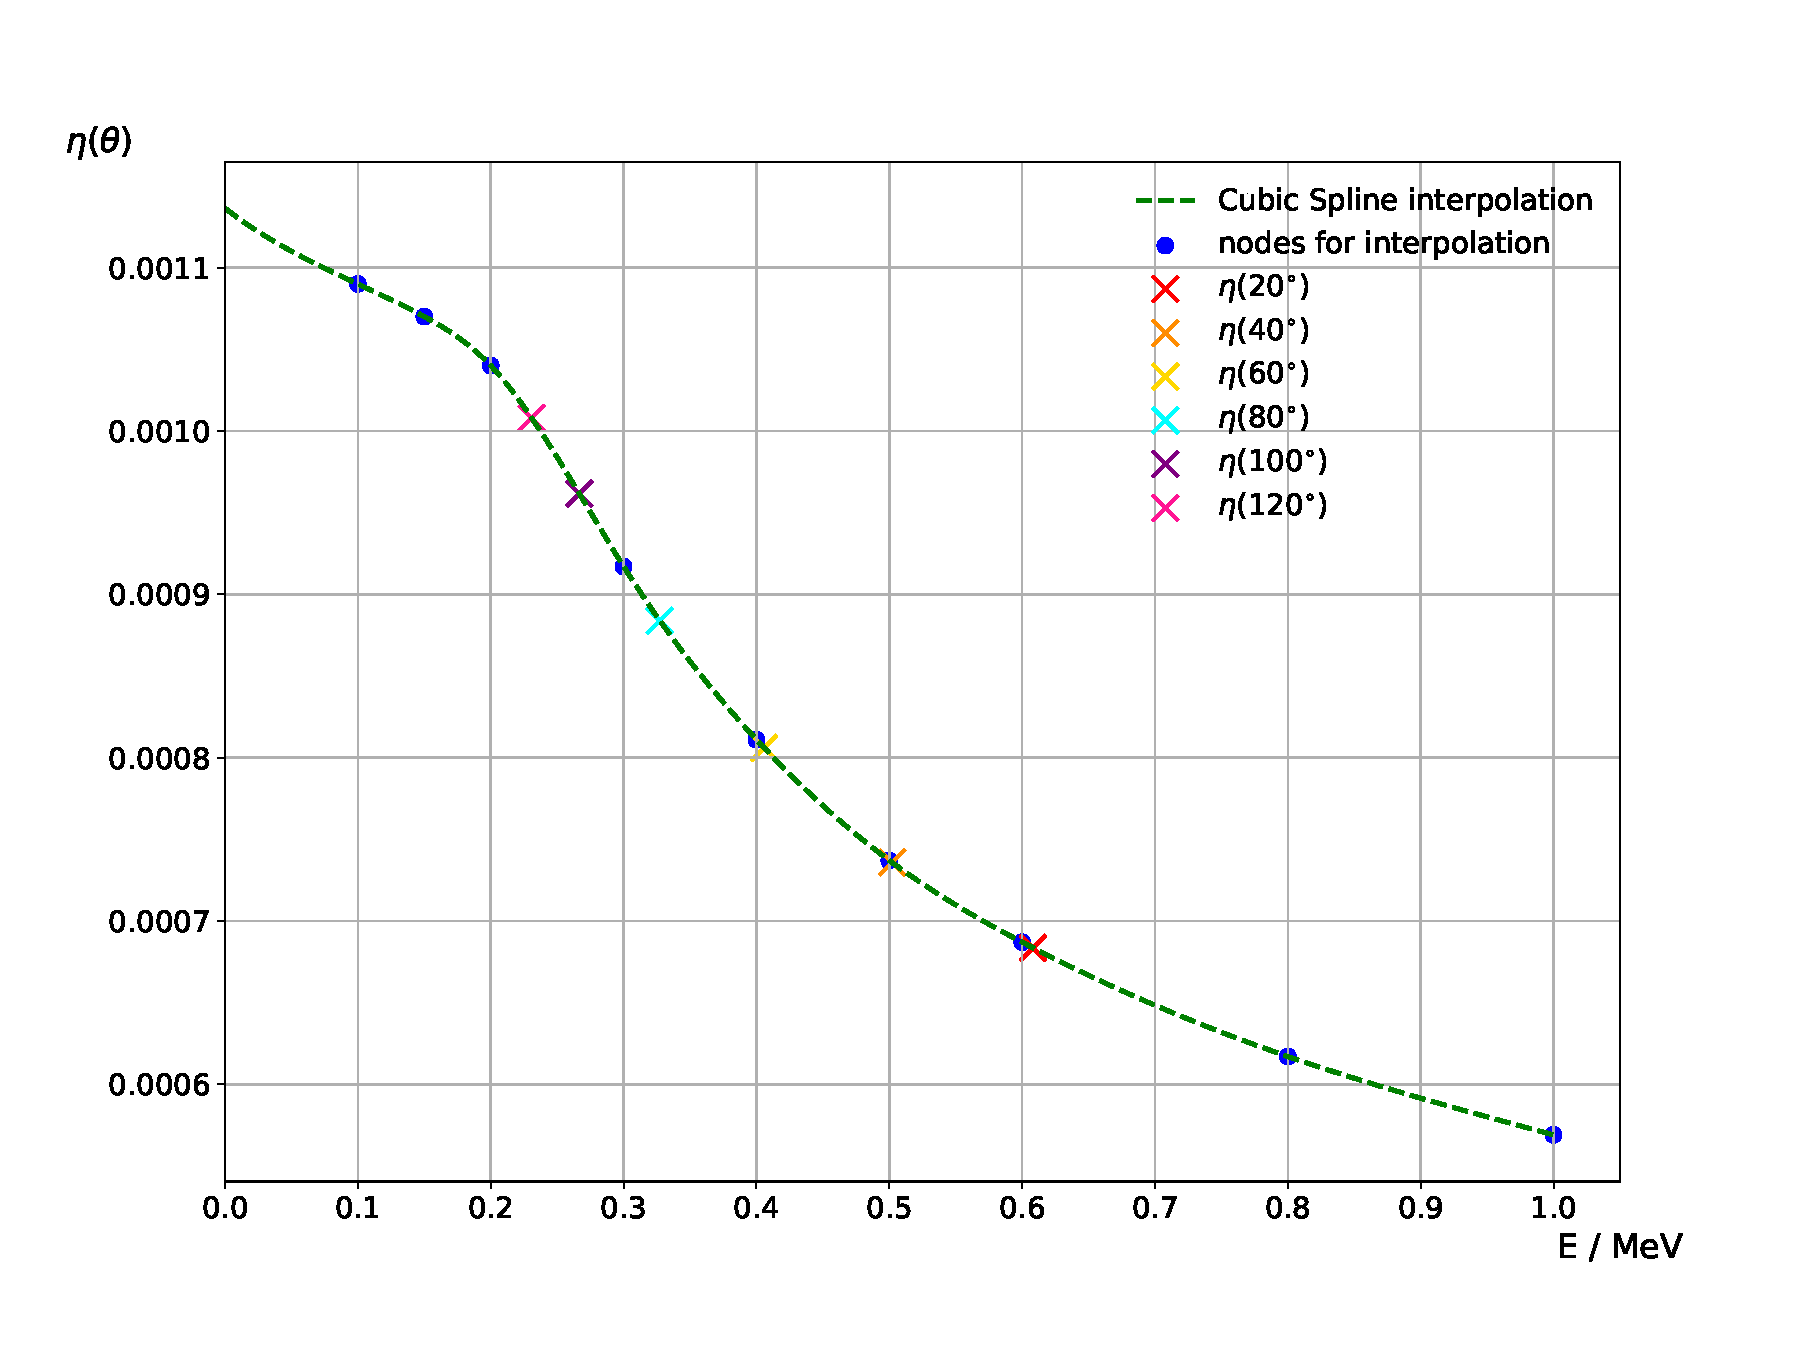
\includegraphics[height=12cm, width=16cm]{images/phyex2_fig1.pdf}
 \label{fig:fig2}
\end{figure}
\item 
我们再利用\textbf{表\ref{tab:table4}}作三次样条函数内插得到连续函数关系如\textbf{图\ref{fig:fig3}}.
\begin{table}[H]
\caption{\textbf{距点源30mm,$\phi$40$\times$40mm NaI(Tl)对点源的峰总比与能量关系}}
\label{tab:table4}
\begin{center}
\setlength{\tabcolsep}{3mm}
\begin{tabular}{|c|c|c|c|c|c|c|c|c|c|}%p{6cm}|}
    \toprule
	\hline
	\textbf{E/MeV} & 0.2 & 0.3 & 0.4 & 0.5 & 0.6 & 0.662 & 0.8 & 1.0\\ \hline
	$\bm{R(\theta)}$ & 0.8841 & 0.7236 & 0.5875 & 0.4912 & 0.4266 & 0.3914 & 0.3373 & 0.2977\\ \hline
	\bottomrule
	\end{tabular}
\end{center}
\end{table}
\begin{figure}[H]
 \centering
 \caption{三次样条函数内插$R(\theta)-E$关系曲线}
 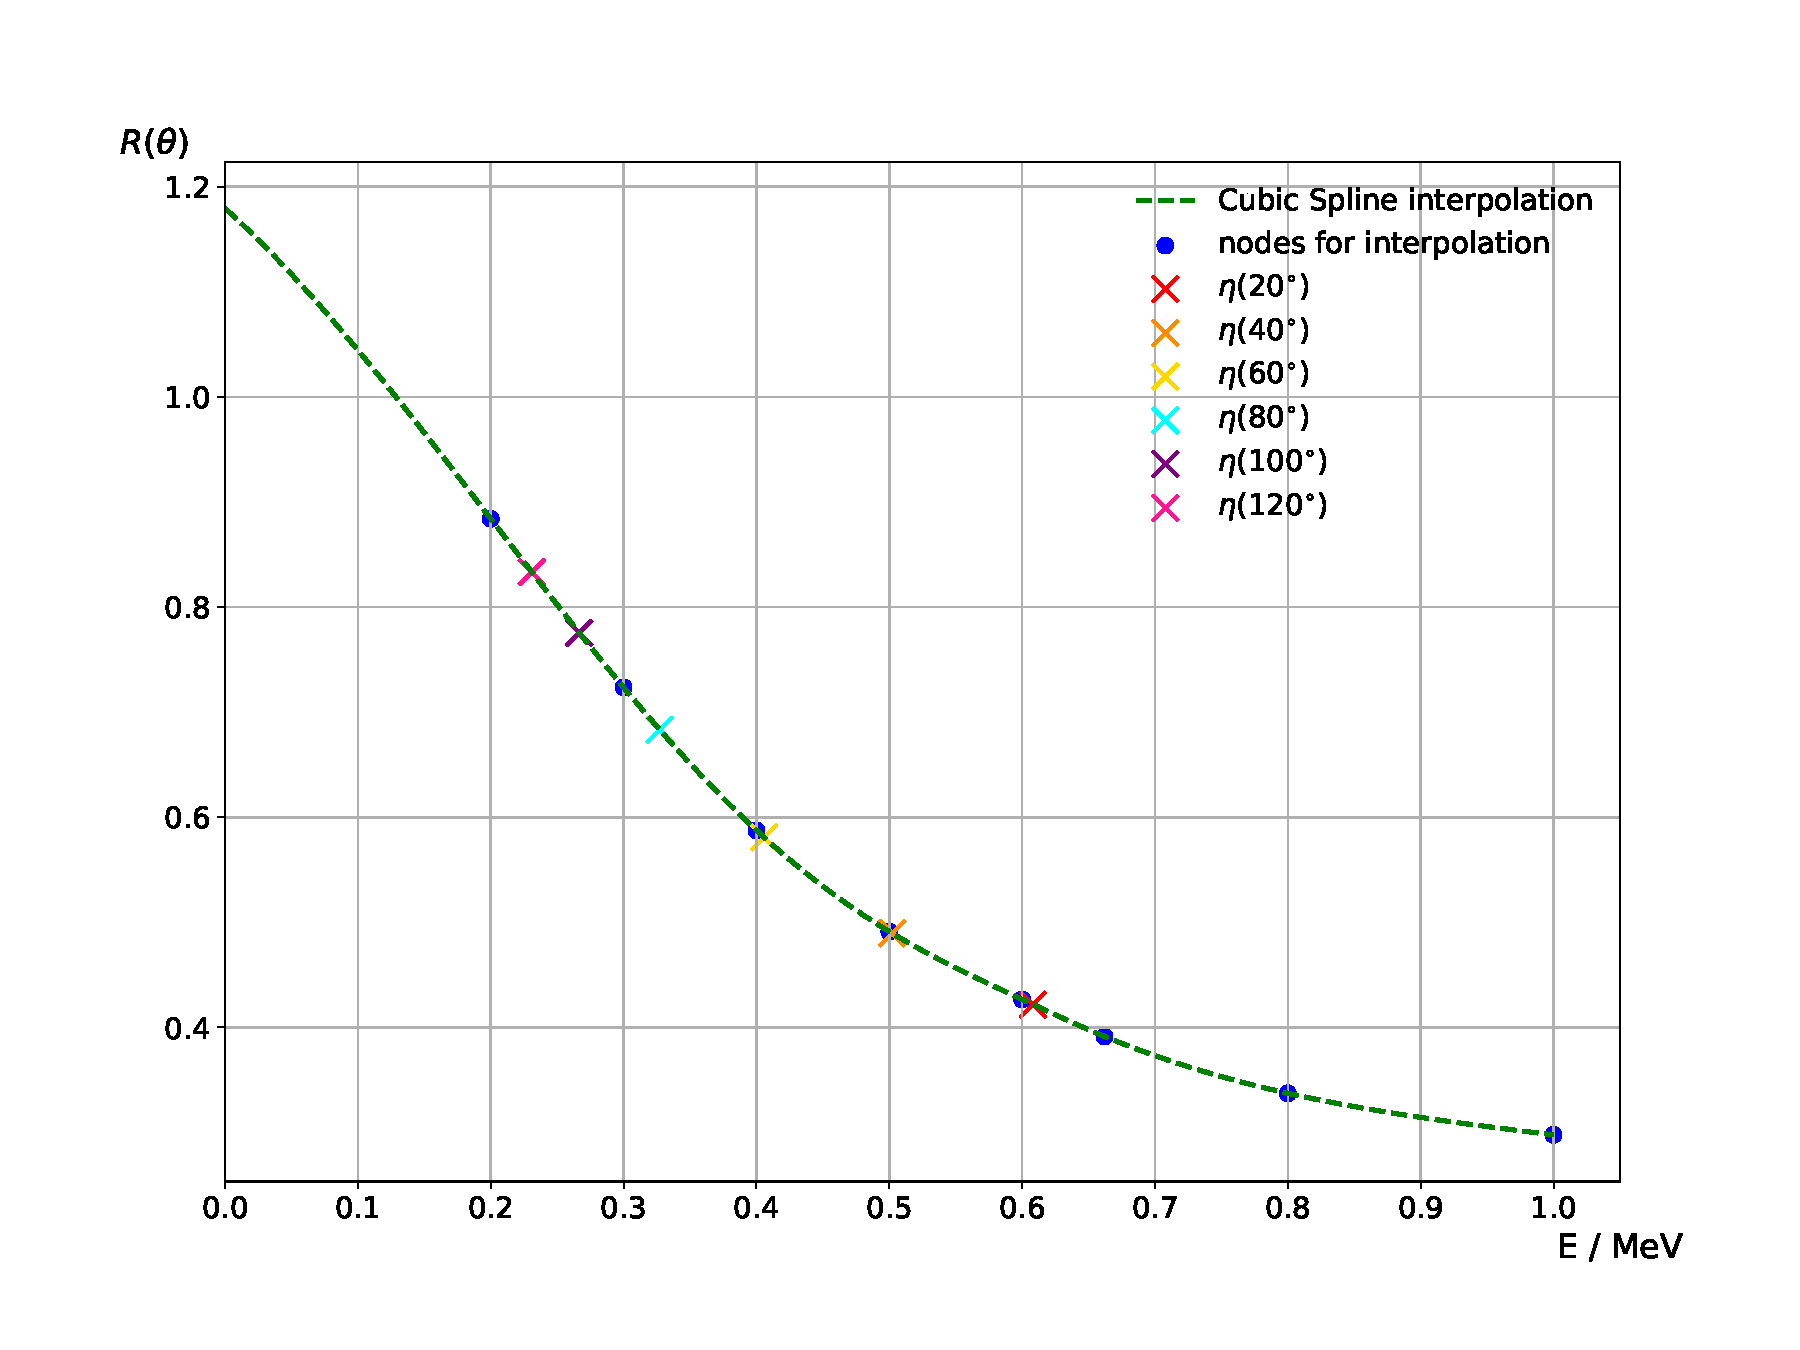
\includegraphics[height=12cm, width=16cm]{images/phyex2_fig2.pdf}
 \label{fig:fig3}
\end{figure}
\item 
通过内插和计算得到结果如下\textbf{表\ref{tab:table5}.}
\begin{table}[H]
\caption{}
\label{tab:table5}
\begin{center}
\setlength{\tabcolsep}{3mm}
\begin{tabular}{|c|c|c|c|c|c|c|}%p{6cm}|}
    \toprule
	\hline
    $\bm{\theta}$ & \textbf{峰位} & \textbf{E/MeV} & $\bm{\eta(\theta)}$ & $\bm{R(\theta)}$ & \textbf{净峰面积} & \textbf{相对微分截面}\\ \hline \hline
	$20^{\circ}$ & 427 & 0.608185 & 0.000683534 & 0.421784 & 22836 & 1\\ \hline
	$40^{\circ}$ & 350 & 0.502156 & 0.000735704 & 0.489555 & 17507 & 0.613673\\ \hline
	$60^{\circ}$ & 280 & 0.405766 & 0.000805984 & 0.580819 & 13412 & 0.361706\\ \hline
	$80^{\circ}$ & 223 & 0.327277 & 0.000883861 & 0.68316 & 12134 & 0.253705\\ \hline
	$100^{\circ}$ & 179 & 0.266689 & 0.000961567 & 0.775486 & 12529 & 0.212126\\ \hline
	$120^{\circ}$ & 153 & 0.230887 & 0.00100792 & 0.833335 & 14563 & 0.218894\\ \hline
	\bottomrule
	\end{tabular}
\end{center}
\end{table}
\item 
我们可以首先求出$\mathrm \sideset{^{137}}{}Cs$的散射散射$\gamma$光子的能量与散射角$\theta$的关系并与实验结果比较,如\textbf{图\ref{fig:fig4}}所示:
\begin{figure}[H]
 \centering
 \caption{$\mathrm \sideset{^{137}}{}Cs$的散射$\gamma$光子的能量与散射角度$\theta$的关系}
 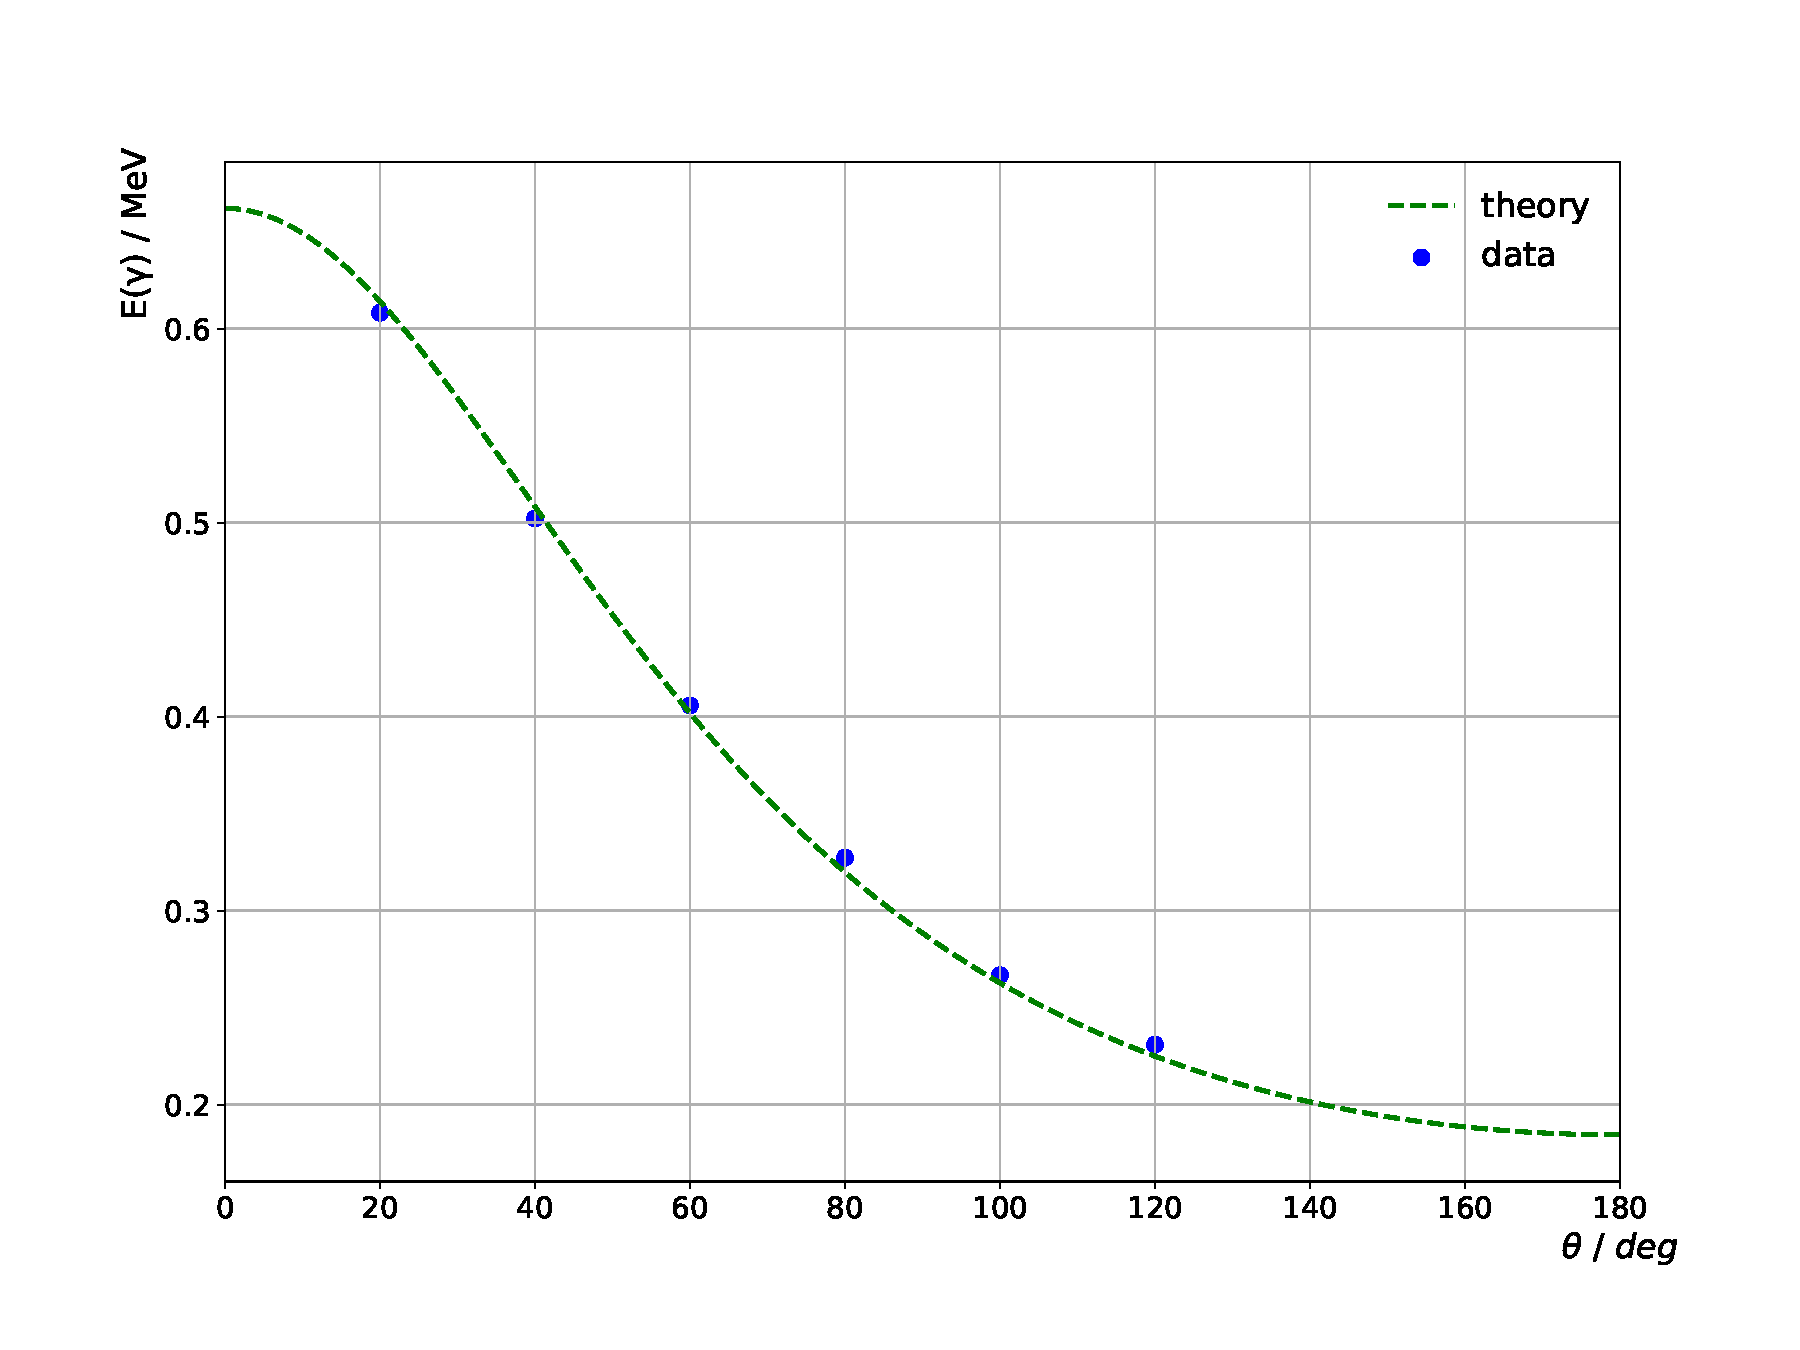
\includegraphics[height=10.5cm, width=14cm]{images/phyex2_fig3.pdf}
 \label{fig:fig4}
\end{figure}
\item 
我们接着可以求出$\mathrm \sideset{^{137}}{}Cs$的散射$\gamma$光子微分散射截面与散射角$\theta$的关系并与实验结果比较,如\textbf{图\ref{fig:fig5}}所示:
\begin{figure}[H]
 \centering
 \caption{$\mathrm  \sideset{^{137}}{}Cs$的散射$\gamma$光子的微分散射截面与散射角度$\theta$的关系}
 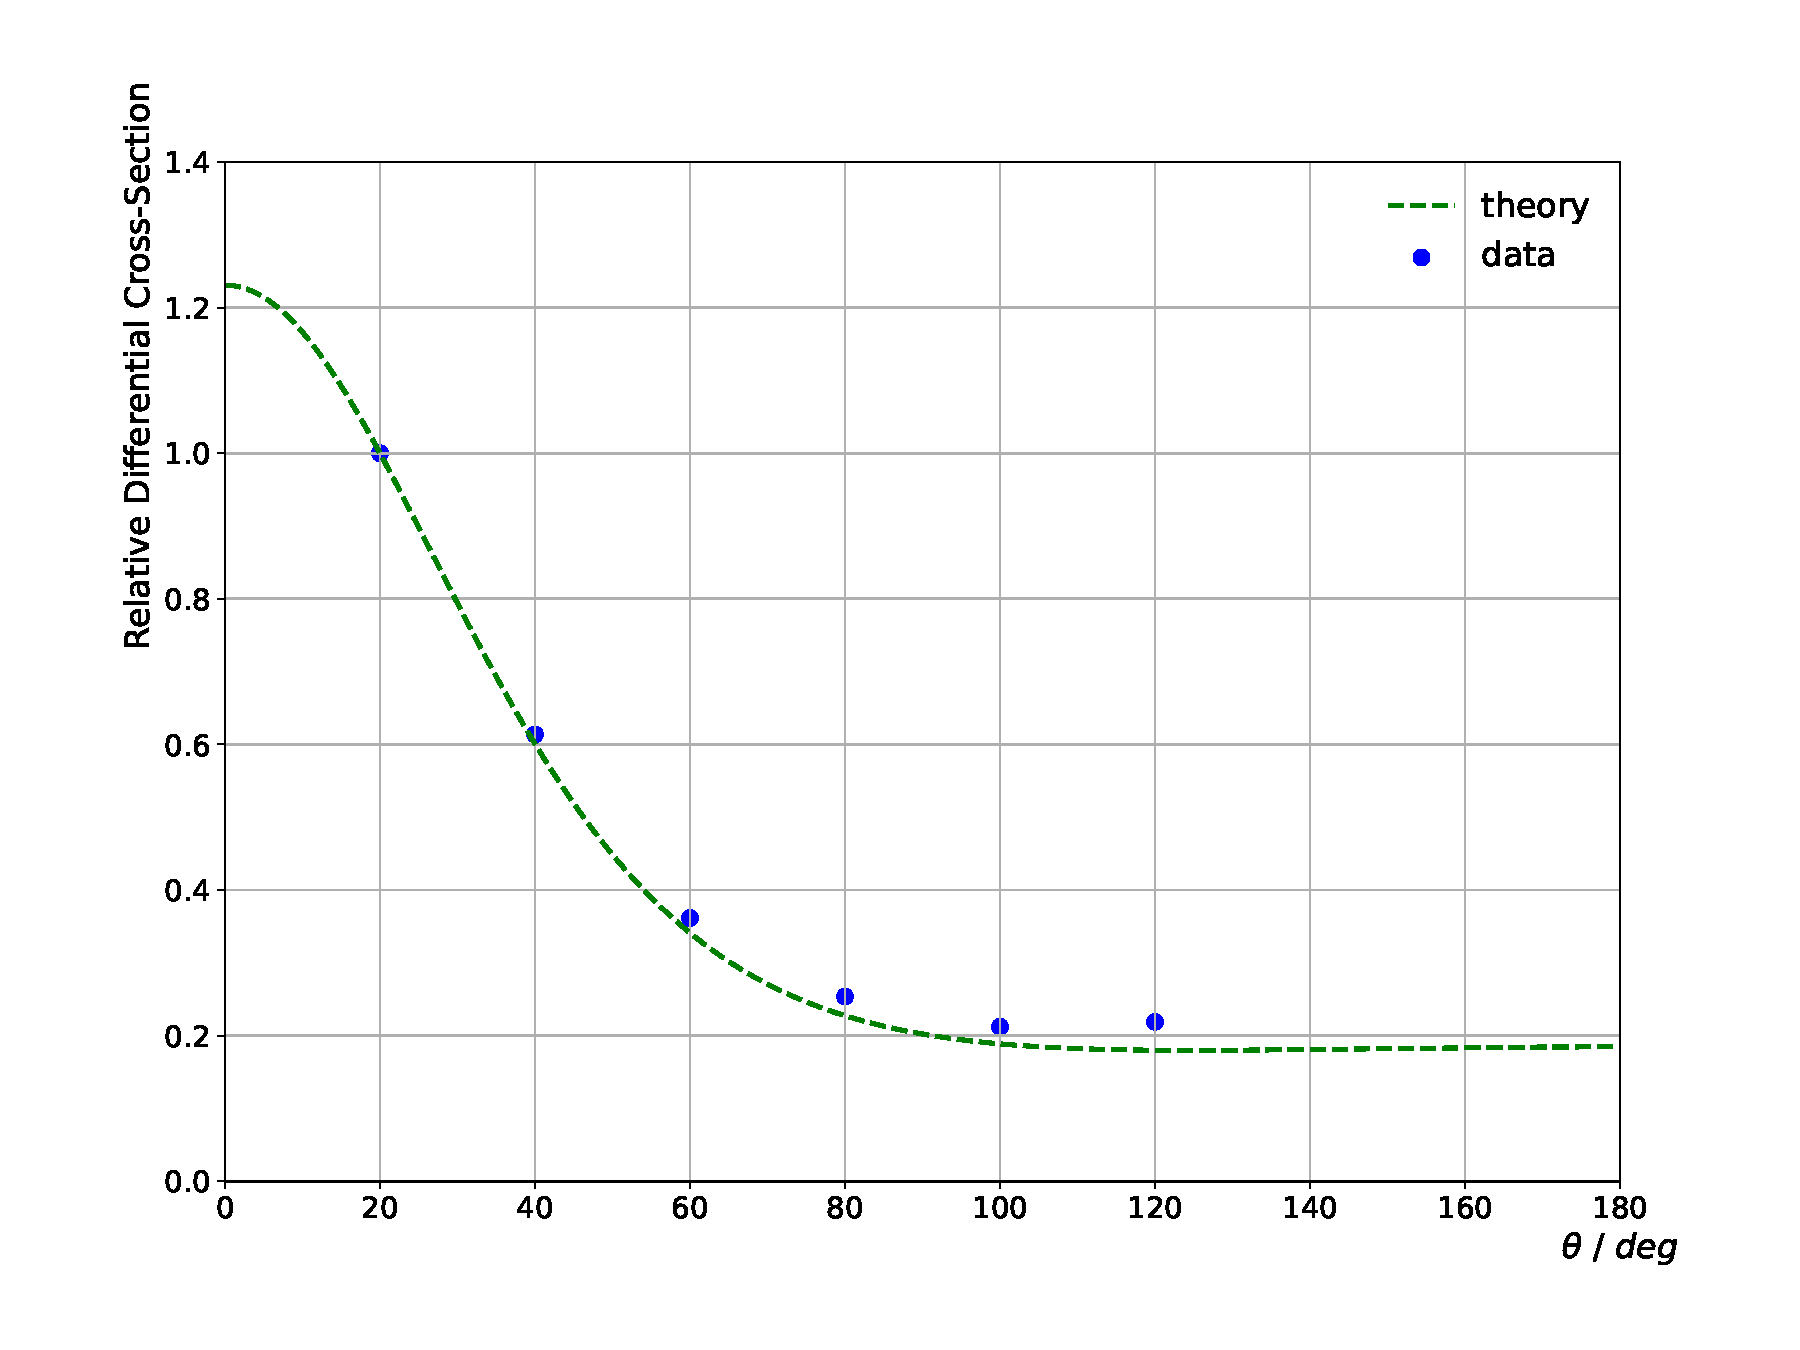
\includegraphics[height=10.5cm, width=14cm]{images/phyex2_fig4.pdf}
 \label{fig:fig5}
\end{figure}
\item 
综上,我们总结上述理论值与实验值的比较结果与误差,展示如下\textbf{表\ref{tab:table6}.}
\begin{table}[H]
\caption{}
\label{tab:table6}
\begin{center}
\setlength{\tabcolsep}{3mm}
\begin{tabular}{|c|c c|c c|}%p{6cm}|}
    \toprule
	\hline
    $\bm{\theta}$ & \textbf{散射光子能量}$\rm E(\gamma)/MeV$ & \textbf{与理论值误差} & \textbf{相对散射截面} & \textbf{与理论值误差}\\ \hline \hline
	$20^{\circ}$ & 0.608185 & -0.95\% & 1 & \diagbox[]{}{}\\ \hline
	$40^{\circ}$ & 0.502156 & -1.15\% & 0.613673 & +2.16\%\\ \hline
	$60^{\circ}$ & 0.405766 & +1.00\% & 0.361706 & +6.05\%\\ \hline
	$80^{\circ}$ & 0.327277 & +2.36\% & 0.253705 & +11.60\%\\ \hline
	$100^{\circ}$ & 0.266689 & +1.54\% & 0.212126 & +12.44\%\\ \hline
	$120^{\circ}$ & 0.230887 & +2.65\% & 0.203863 & +13.29\%\\ \hline
	\bottomrule
	\end{tabular}
\end{center}
\end{table}
\end{enumerate}
%%%%%%%%%%%%%%%%%%%%%%%%%%%%%%%%%%%%%%%% Conclusion %%%%%%%%%%%%%%%%%%%%%%%%%%%%%%%%%%%%%%%%
\newpage
\section{结论}\label{conclusions}
本实验以$\mathrm \sideset{^{137}}{}Cs$为放射源,考察了0.662MeV光子散射后的能量角分布及相对微分散射截面角分布,结果与康普顿散射理论的预计基本一致,在误差范围内,可以说是验证了康普顿效应.

同时,实验简要分析了可能的误差来源,提出了周围墙体散射可能带来的显著影响;建
议更为精确的测定应当在尽可能减小二次散射的空旷环境中进行。\\

%%%%%%%%%%%%%%%%%%%%%%%%%%%%%%%%%%%%%%%% Questions %%%%%%%%%%%%%%%%%%%%%%%%%%%%%%%%%%%%%%%%
\section{实验报告思考题}\label{questions}
\subsection{分析本实验的主要误差来源,试述有限立体角的影响和减少实验误差的办法}\label{sub:question1}
答:减少实验误差:本实验中仅取3点标定了系统的能量刻度,相
应的线性拟合结果虽具有充分大的相关性系数,但其误差显著,不可忽略;后续可采
用更丰富的峰值数据进行定标,以提升能量刻度的准确性.
\subsection{讨论实验值与理论值不完全符合的原因}\label{sub:question2}
答:据图线和数据可知,实测能量较理论值普遍有偏差,但偏差不甚显著;而相对截面
的偏差则比较显著.简要分析可知,上述偏差应当主要源于实验
环境的非理想性;事实上,本实验中有诸多误差来源未能充分控制:\\
a.首先,能量刻度可能不够精准,而关于怎么减少能量刻度误差的办法,可以参考上一问.\\
b.此外,仪器附近物质中的电子均可参与散射过程,而本实验所在的室内环境不甚空旷,势必对散射能谱造成影响.这一影响并不能通过去除本底而完全消除;事实上,加上铝棒后,散射导致光子的角分布比未加铝棒时显著增大,从而四壁对光子的散射效应增强、角分布更广,导致了额外的散射截面.
\\


%%%%%%%%%%%%%%%%%%%%%%%%%%%%%%%%%%%%%%%% Acknowledgements %%%%%%%%%%%%%%%%%%%%%%%%%%%%%%%%%%%%%%%%

\section{致谢}\label{acknowledgments}
感谢楼建玲老师在实验中的的悉心指导.

%%%%%%%%%%%%%%%%%%%%%%%%%%%%%%%%%%%%%%%% Cite %%%%%%%%%%%%%%%%%%%%%%%%%%%%%%%%%%%%%%%%
\begin{comment}
如果需要索引参考文献,请使用\cite{Erdos01}, 同时已经将参考文献的项目模版在文末写出。
\end{comment}

\begin{comment}
%%%%%%%%%%%%%%%%%%%%%%%%%%%%%%%%%%%%%%%% Appendix %%%%%%%%%%%%%%%%%%%%%%%%%%%%%%%%%%%%%%%%
\appendix
\section{代码}\label{sub:app.code}
请在附录\ref{sub:app.code}中添加代码。请使用如下Scala的语法高亮描述方法。
\begin{scala}
class TopIO extends Bundle() {
	val boot = Input(Bool()) 
// imem and dmem interface for Tests
	val test_im_wr		= Input(Bool())
	val test_im_rd 		= Input(Bool())
	val test_im_addr 	= Input(UInt(32.W))
	val test_im_in 		= Input(UInt(32.W))
	val test_im_out 	= Output(UInt(32.W))

	val test_dm_wr		= Input(Bool())
	val test_dm_rd 		= Input(Bool())
	val test_dm_addr 	= Input(UInt(32.W))
	val test_dm_in 		= Input(UInt(32.W))
	val test_dm_out 	= Output(UInt(32.W))

	val valid			= Output(Bool())
}
class Top extends Module() {
	val io 		= IO(new TopIO())//in chisel3, io must be wrapped in IO(...) 
	//...
	when (io.boot & io.test_im_wr){
		imm(io.test_im_addr) := io.test_im_in
		} .elsewhen (io.boot & io.test_dm_wr){
		// please finish it
		} //...
}
\end{scala}
\newpage

%%%%%%%%%%%%%%%%%%%%%%%%%%%%%%%%%%%%%%%% REFERENCE %%%%%%%%%%%%%%%%%%%%%%%%%%%%%%%%%%%%%%%%
\begin{thebibliography}{9}

\bibitem{Erdos01} P. Erd\H os, \emph{A selection of problems and
results in combinatorics}, Recent trends in combinatorics (Matrahaza,
1995), Cambridge Univ. Press, Cambridge, 2001, pp. 1--6.

\end{thebibliography}
\end{comment}
\end{document}

